\documentclass[11pt,letterpaper]{article}
\usepackage[T1]{fontenc}
\usepackage{lmodern,microtype}
\usepackage[margin=0.82in,headheight=15pt]{geometry}
\usepackage{graphicx,booktabs,longtable,array,tabularx}
\usepackage[dvipsnames]{xcolor}
\usepackage{listings,enumitem,fancyhdr,titlesec}
\usepackage{tikz}
\usetikzlibrary{arrows.meta,positioning,fit}
\usepackage{hyperref,xurl,seqsplit}
\hypersetup{hypertexnames=false,colorlinks=true,linkcolor=MidnightBlue,urlcolor=MidnightBlue,citecolor=MidnightBlue,
 pdftitle={IA-840F OFS 2026.1 and AHLS Support Guide},pdfauthor={IA-840F project},
 pdfsubject={Zero-to-vector-add setup with Quartus 26.1, AHLS 2026.1 and OPAE 2.14.0-3}}
\definecolor{GuideBlue}{HTML}{173B56}
\definecolor{CodeGray}{HTML}{F3F5F7}
\definecolor{RuleGray}{HTML}{C7CED5}
\setlength{\parindent}{0pt}
\setlength{\parskip}{6pt}
\setlist{itemsep=3pt,topsep=4pt,leftmargin=*}
\titleformat{\section}{\Large\bfseries\color{GuideBlue}}{\thesection}{0.6em}{}
\titleformat{\subsection}{\large\bfseries\color{GuideBlue}}{\thesubsection}{0.6em}{}
\titleformat{\subsubsection}{\normalsize\bfseries}{\thesubsubsection}{0.6em}{}
\pagestyle{fancy}
\fancyhf{}
\fancyhead[L]{\small IA-840F \textbar\ OFS 2026.1 / AHLS}
\fancyhead[R]{\small User support guide}
\fancyfoot[L]{\small Project release documentation}
\fancyfoot[R]{\thepage}
\renewcommand{\headrulewidth}{0.3pt}
\newcommand{\code}[1]{{\ttfamily\expandafter\seqsplit\expandafter{\detokenize{#1}}}}
\newcommand{\src}[1]{\cite{S#1}}
\newcommand{\stepnote}[2]{\begin{quote}\small\textbf{#1.} #2\end{quote}}
\newcommand{\chapterstart}[1]{\clearpage\section{#1}}
\lstdefinestyle{shell}{basicstyle=\ttfamily\footnotesize,backgroundcolor=\color{CodeGray},
 frame=single,rulecolor=\color{RuleGray},framerule=0.3pt,framesep=6pt,
 columns=fullflexible,keepspaces=true,showstringspaces=false,breaklines=true,
 breakatwhitespace=false,postbreak=\mbox{\textcolor{GuideBlue}{\tiny continuation}\space},
 upquote=true,aboveskip=8pt,belowskip=8pt}
\lstset{style=shell}
\newcolumntype{Y}{>{\raggedright\arraybackslash}X}
\begin{document}
\begin{titlepage}
\vspace*{0.5in}
{\large\color{GuideBlue} IA-840F platform documentation\par}
\vspace{0.35in}
{\Huge\bfseries IA-840F\par}
\vspace{0.12in}
{\LARGE\bfseries OFS 2026.1 and AHLS\par Support Guide\par}
\vspace{0.4in}
{\Large From a new Linux installation to\par building and running SYCL vector-add\par}
\vspace{0.45in}
\par\noindent\begin{tabularx}{\linewidth}{@{}p{0.38\linewidth}Y@{}}
\toprule
FPGA platform & BittWare IA-840F, Agilex 7, \code{AGFB027R25A2E2V}\\
Static platform & OFS \code{ofs-2026.1-1} FIM and matching PIM/PR collateral\\
FPGA implementation & Quartus Prime Pro 26.1.1 Build 130 (26.1 family)\\
Compiler/runtime & Altera HLS IP Gen (AHLS) 2026.1.0\\
Host access stack & Latest published OFS OPAE release \textbf{2.14.0-3}\\
Board package & Current IA-840F oneAPI Accelerator Support Package\\
Document revision & 8 October 2026\\
\bottomrule
\end{tabularx}\par
\vfill
\textbf{Scope}\par
A practical, version-pinned guide for the current project stack. It covers one-time
host and board preparation, the normal compiler-driven BSP link, the four
standard/USM and plain/kclk configurations, and a verified prebuilt-image path.

This is project documentation, not an official BittWare or Altera publication.
The supplied BittWare support guide informed the chapter structure; its older
installation and programming recipes are not substituted for this stack.\src{1}
\end{titlepage}
\pagenumbering{roman}
\tableofcontents
\clearpage
\section*{Read this before starting}
\addcontentsline{toc}{section}{Read this before starting}
\textbf{One-time setup and routine application work are different operations.}
A new host needs the Linux access stack, toolchain, board power/cooling and a
matching static FIM. Once those are correct, vector-add compilation and an AFU
partial-reconfiguration load do not require another full-device flash or a
workstation reboot.

\textbf{Two routes are documented.} The full hardware build compiles your SYCL
kernel into a new image. The prebuilt route links the supplied, already-fitted
program through the actual AHLS driver, then runs that image. Use the latter for
an initial full-oracle numerical bring-up without spending another FPGA fit;
use the former when changing device code. Both produce a real SYCL \code{.fpga}
fat binary, not a raw-AFU replacement host.\src{11}

\textbf{The main instructions target one coherent current stack.} OPAE is pinned
to the latest published release, \code{2.14.0-3}, commit
\path{e4b329185d2c462f5b8c3c74443a5c5cdb25f3b3}. This is a deliberate release pin,
not an instruction to track a moving development branch.\src{17}

\textbf{Commands are recipes, not permission to run a dangerous operation.}
Perform remote workstation work in an owned \code{tmux} session. Resolve the
actual card, BDFs, IOMMU groups and current ownership before an operation that
opens the accelerator, programs an image, creates a VF or changes power.
An unknown process or timed-out hardware access is a stop condition, not a
reason for another reset, PR load or probe.\src{10}

\textbf{Obtain the complete input set.} The ASP archive includes the application
images and compiler PR template. It is not itself a factory-card cold-boot flash
package. A factory-programmed card additionally needs the matched, verified
full-device FIM provisioning bundle described in Section~\ref{sec:fim}.\src{8}

\stepnote{Copying commands}{Define the path variables in Section~\ref{sec:paths}
first. Replace example hardware identifiers only with identifiers verified for
your host. Wrapped listings display a small ``continuation'' marker; it is a
layout aid, not a token to enter in a shell.}
\clearpage
\pagenumbering{arabic}
\section{Overview and included configurations}
\label{sec:overview}
\subsection{What the stack does}
AHLS compiles SYCL device code and supplies the \code{kernel_system}. The
oneAPI ASP provides board-facing kernel, memory, CSR, clock/reset and runtime
integration. The ASP and generated kernel together form the application AFU
inside the static FIM's PR region. PIM adapts the AFU to the FIM interfaces; it
is not a separately loaded application tier. On the host, SYCL/OpenCL reaches
the accelerator through MMD/MPF, OPAE and the Linux DFL/VFIO drivers.\src{3}

\begin{center}
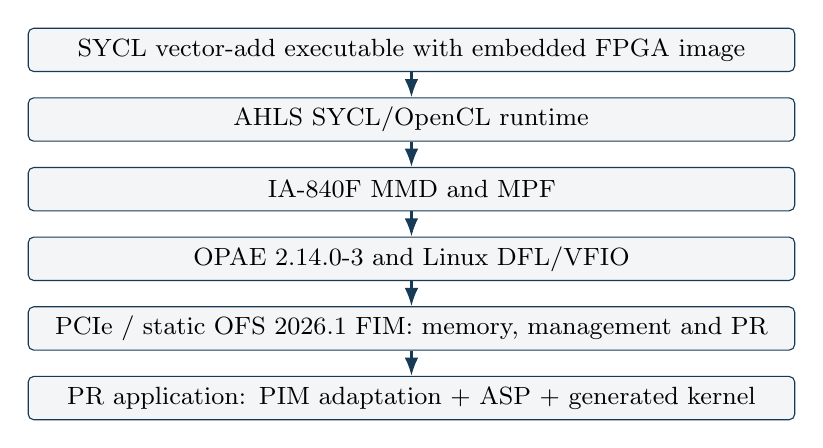
\begin{tikzpicture}[node distance=0.32cm,box/.style={draw=GuideBlue,rounded corners=2pt,
 fill=CodeGray,text width=9.5cm,align=center,minimum height=0.55cm,font=\small},
 arrow/.style={-{Latex},draw=GuideBlue,thick}]
\node[box] (app) {SYCL vector-add executable with embedded FPGA image};
\node[box,below=of app] (sycl) {AHLS SYCL/OpenCL runtime};
\node[box,below=of sycl] (mmd) {IA-840F MMD and MPF};
\node[box,below=of mmd] (opae) {OPAE 2.14.0-3 and Linux DFL/VFIO};
\node[box,below=of opae] (fim) {PCIe / static OFS 2026.1 FIM: memory, management and PR};
\node[box,below=of fim] (afu) {PR application: PIM adaptation + ASP + generated kernel};
\foreach \a/\b in {app/sycl,sycl/mmd,mmd/opae,opae/fim,fim/afu} \draw[arrow] (\a)--(\b);
\end{tikzpicture}
\end{center}
\textit{Logical software/hardware path, not a physical floorplan or a latency diagram.}

\subsection{Variants and compile flows}
\par\noindent\begin{tabularx}{\linewidth}{@{}l l Y@{}}
\toprule
Variant & Flow & Intended use\\\midrule
\code{ofs_ia840f} & \code{afu_flat} & Standard local-memory/buffer path. Start here.\\
\code{ofs_ia840f} & \code{afu_flat_kclk} & Same memory variant with the kernel-clock/PIM-CDC alternative.\\
\code{ofs_ia840f_usm} & \code{afu_flat} & USM-enabled variant; the example uses shared USM.\\
\code{ofs_ia840f_usm} & \code{afu_flat_kclk} & USM with the alternate clock topology.\\
\bottomrule
\end{tabularx}\par

Both variants target the same IA-840F part and two 16-GiB local DDR banks
(32 GiB aggregate). The USM variant adds the host/shared-memory path. The
\code{_kclk} choice enables \code{USE_KERNEL_CLK_EVERYWHERE_IN_PR_REGION} in the
PR integration and changes its PIM CDC/domain configuration; it does not
change the static PCIe or DDR reference clocks. Output revision names alone
are not proof of topology.\src{20}

\subsection{Version and identity contract}
The static FME interface UUID is
\path{fc603c44-5c8f-5e94-bcbe-a5780030947c}. The standard and USM AFU UUIDs are
\path{51ED2F4A-FEA2-4261-A595-918500575509} and
\path{5D9FEF7B-C491-4DCE-95FC-F979F6F061BE}, respectively. FME and AFU UUIDs
serve different roles. A matching AFU UUID is not enough to identify the
physical card, and the two compile flows of one variant share an AFU UUID.\src{20}

The package is a project-qualified IA-840F port of current OFS ASP machinery.
A stock N6001 board package, an unrelated static QDB, or an older vendor BSP
is not an interchangeable dependency.\src{20}

\chapterstart{Inputs, workspace and host prerequisites}
\label{sec:paths}
\subsection{Required files}
Obtain these inputs before installation. Licensed tools and full-device
programming images are separate from a source checkout.
\par\noindent\begin{tabularx}{\linewidth}{@{}p{0.38\linewidth}Y@{}}
\toprule
Input & Purpose\\\midrule
Quartus Pro 26.1.1 + Agilex 7 support & FPGA implementation and programming-file tools.\\
AHLS 2026.1.0 distribution/helper & Compiler, SYCL/OpenCL runtime and FPGA tools.\\
Valid Quartus entitlement & Required for the implementation operations you use.\\
BittWare SDK 2026.1 EL9 package & Current IA-840F management/product support.\\
OPAE \code{2.14.0-3} sources & Host libraries, plugins, utilities and platform tools.\\
IA-840F ASP release archive & Current compiler metadata, RTL, runtime and four image sets.\\
Paired FIM provisioning bundle & Full-device SOF/RPD/MAP and recovery material for a factory card.\\
Matching PR platform/template & The accepted static QDB and PIM/compiler collateral.\\
\bottomrule
\end{tabularx}\par
The latest OPAE release is available at
\url{https://github.com/OFS/opae-sdk/releases/tag/2.14.0-3}.\src{17}
Obtain the proprietary SDK and board-revision hardware documentation from the
BittWare developer distribution; do not invent a download URL or reuse a
package intended for a different board.

\subsection{Use explicit paths}
These variables are used throughout the guide. The example layout keeps
sources, tools, build trees and logs separate.
\begin{lstlisting}[language=bash]
WORK="$HOME/ia840f-work"
DOWNLOADS="$WORK/downloads"
AHLS="$HOME/ahls/altera_hls/aclsycl"
QUARTUS="/opt/altera/26.1.1/quartus"
BSP="$WORK/asp/ia840f"
OPAE_SRC="$WORK/src/opae-sdk"
OPAE_BUILD="$WORK/build/opae"
OPAE_PREFIX="$WORK/install/opae"
PR="$BSP/pr_build_template"
mkdir -p "$DOWNLOADS" "$WORK/src" "$WORK/build" "$WORK/logs"
tmux new-session -s ia840f-setup
\end{lstlisting}
Run the remaining workstation commands inside that session. The unpacked
\code{BSP} must be writable by its operator because private runtime activation
creates prefix-specific FCD/ICD files. \code{PR} can instead name a separately
supplied, matching accepted PR export; do not point it at arbitrary FIM source.

\subsection{Host, power and cooling}
The qualified host uses Rocky Linux 9.8, x86-64, kernel
\code{5.14.0-687.48.1.el9_8.x86_64}; its compatible DFL modules are exposed
through enterprise \code{weak-updates}. This is project validation, not a claim
that every distribution is vendor-certified.\src{5}

Install the card, auxiliary power and cooling according to the hardware guide
for the physical board revision. Power the host down before physical
installation. The PCIe slot alone is not a substitute for the required
auxiliary supply. USB IN is useful for BMC management/provisioning; it is not
required for routine PCIe PR merely because a historical guide used JTAG.
The qualification workstation negotiates Gen3 x16; do not attempt unrelated
link retraining to force a Gen4 result.

\subsection{BIOS, IOMMU and huge pages}
Enable the host's IOMMU/virtualization and SR-IOV features. Use a deliberate
Secure Boot/module-signing policy: unsigned out-of-tree modules require a
compatible policy, not an automatic security bypass. The verified host reserves
2048 two-MiB huge pages and enables Intel IOMMU and PCI resource reallocation.\src{5}
For the Intel/Rocky qualification configuration:
\begin{lstlisting}[language=bash]
sudo grubby --update-kernel=ALL \
  --args='intel_iommu=on pci=realloc hugepagesz=2M hugepages=2048'
# Reboot only after completing the intended host setup and saving work.
# After returning to an owned tmux session:
cat /proc/cmdline
grep -E '^HugePages_|^Hugepagesize:' /proc/meminfo
\end{lstlisting}
Use the appropriate IOMMU option for another CPU platform; do not copy
\code{intel_iommu} onto a different architecture without checking its Linux
support. The huge-page reservation is a setup choice, not proof that allocation
and access work; the numerical run is the verification step.

\subsection{Build resources and limits}
CMake 3.20 or later is required by the BSP/sample targets. The observed
qualification host has approximately 125 GiB usable RAM. That observation is
not an Altera minimum specification. Use live headroom to admit builds and
reserve a 55-GiB per-process virtual-address-space limit:
\begin{lstlisting}[language=bash]
ulimit -v 57671680
free -h
df -h "$WORK"
\end{lstlisting}
At most two fits run simultaneously in this workflow. A per-process virtual
limit does not constrain aggregate RSS or all children as one budget. A
prebuilt image link is much smaller than a full fit.

\chapterstart{Installing the current software stack}
\label{sec:install}
\subsection{System build dependencies}
On a new Rocky host, install the build dependencies through the configured
Rocky repositories. Review the transaction before accepting it:
\begin{lstlisting}[language=bash]
sudo dnf install \
  gcc gcc-c++ make cmake git tmux tar gzip unzip \
  python3 python3-pip python3-devel \
  libuuid-devel json-c-devel libedit-devel \
  numactl-devel hwloc-devel tbb-devel \
  openssl-devel libffi-devel pkgconf-pkg-config
\end{lstlisting}
DFL source builds additionally require headers/development files matching the
running kernel. AHLS helper prerequisites include \code{rpm2cpio} and
\code{uidmap}; use the appropriate distribution packages/provider for those
commands.\src{2}
Do not import an unrelated repository key or disable signature checks to work
around a failing optional repository. Scope an individual package operation to
the already-configured official repositories when necessary.

\subsection{Quartus Prime Pro 26.1.1}
Install Quartus Pro 26.1.1 Build 130 and Agilex 7 device support in a distinct
prefix. Obtain the licensed installer from Altera, inspect its actual help,
and select the correct device family. Existing versions may remain installed;
this guide selects the build tool explicitly rather than changing the login
shell's global default.\src{20}

For Altera's qinst/Makeself installer, pass qinst arguments after the wrapper's
\code{--} separator. A representative component selection is:
\begin{lstlisting}[language=bash]
QINST="/absolute/path/to/the/downloaded/qinst-installer.run"
"$QINST" --help
sudo "$QINST" --noprogress --nox11 -- \
  --cli --accept-eula \
  --download-dir "$DOWNLOADS/quartus" \
  --install-dir /opt/altera/26.1.1 \
  --components quartus,agilex7
# Verify the actual installed version, without a stale override:
env -u QUARTUS_ROOTDIR_OVERRIDE \
  "$QUARTUS/bin/quartus_sh" --version
\end{lstlisting}
The precise downloaded installer filename and entitlement are supplied by your
software distribution. Questa is optional for the hardware vector-add route;
install the matched FPGA Edition if you separately require simulation. Set
\code{LM_LICENSE_FILE} to your valid entitlement/server without placing license
contents or credentials in this guide.

\subsection{AHLS 2026.1.0}
The Altera installation helper can install or reuse Quartus and construct an
Apptainer-based development environment. Its interactive prompts accept the
install directory, Quartus tree/archive and an AHLS package/existing tree
containing \code{aclsycl/fpgavars.sh}.\src{2}
\begin{lstlisting}[language=bash]
cd "$DOWNLOADS"
bash ./ahls-install-helper.sh --help
bash ./ahls-install-helper.sh
# Choose AHLS 2026.1.0, not an unpinned latest compiler.
# For an existing Quartus installation, select /opt/altera/26.1.1.
# Confirm the summary before accepting installation.
\end{lstlisting}
The helper normally creates \code{<install>/bin/ahls-sh}. That shell is useful
for its documented container flow, but the validated ASP application workflow
runs the installed AHLS tools natively on the host after sourcing
\code{fpgavars.sh}. Do not inherit a helper's stale Quartus bind or expect host
OPAE/Python installations to appear automatically inside a container.\src{2}
\begin{lstlisting}[language=bash]
source "$AHLS/fpgavars.sh" >/dev/null
"$AHLS/bin/ahls" --version
test -f "$AHLS/include/sycl/ext/altera/fpga_extensions.hpp"
test -f "$AHLS/host/linux64/lib/libalteracl.so"
\end{lstlisting}
Require AHLS 2026.1.0 Build
\path{461da9be608f74678d9c52a2dc1cbb67c58d57fa}. A version/help result establishes
installation visibility, not a successful FPGA board build.\src{20}

\subsection{BittWare SDK and IA-840F product support}
Install the current EL9 SDK package from the board distribution. The inspected
SDK includes the IA-840F/Agilex product wheel
\code{bw_agilex_product-0.1.49}; product support is not absent merely because an
obsolete separate CSP package is no longer present.\src{6}
\begin{lstlisting}[language=bash]
SDK_RPM="$DOWNLOADS/bittware-sdk-2026.1.0-1.el9.rpm"
rpm --checksig "$SDK_RPM"
sudo dnf install "$SDK_RPM"
sudo usermod -aG bittware "$USER"
# Log out/in when group membership changes.
/usr/share/bittware-sdk/bin/bw_pip install
/usr/share/bittware-sdk/bin/bw_ls
\end{lstlisting}
Use the executable paths printed/installed by your SDK. Management tools and
\code{bittware-vfiod} are required for the selected management operation,
not a reason to start a competing daemon while an application owns the card.

\subsection{OPAE 2.14.0-3: build into an owned prefix}
Clone the official repository and pin the latest published release. The library,
VFIO/UIO plugins and utilities must come from the same installation.\src{17}
\begin{lstlisting}[language=bash]
git clone https://github.com/OFS/opae-sdk.git "$OPAE_SRC"
git -C "$OPAE_SRC" checkout --detach \
  e4b329185d2c462f5b8c3c74443a5c5cdb25f3b3
git -C "$OPAE_SRC" rev-parse HEAD
# The supplied configuration-only patch makes private module selection relocatable.
git -C "$OPAE_SRC" apply --check \
  /path/to/manual-sources/opae214-relocatable-modules.patch
git -C "$OPAE_SRC" apply \
  /path/to/manual-sources/opae214-relocatable-modules.patch
export PIP_IGNORE_INSTALLED=1
cmake -S "$OPAE_SRC" -B "$OPAE_BUILD" \
  -DCMAKE_BUILD_TYPE=Release \
  -DCMAKE_INSTALL_PREFIX="$OPAE_PREFIX" \
  -DCMAKE_INSTALL_LIBDIR=lib64 \
  -DPython3_EXECUTABLE=/usr/bin/python3.9 \
  -DPYTHON_EXECUTABLE=/usr/bin/python3.9 \
  -DOPAE_BUILD_TESTS=OFF -DOPAE_BUILD_LEGACY=OFF \
  -DOPAE_BUILD_EXTRA_TOOLS=ON -DOPAE_BUILD_OPAEIO=ON \
  -DOPAE_BUILD_USERCLK=ON -DOPAE_BUILD_PLUGIN_VFIO=ON \
  -DOPAE_BUILD_LIBOPAEVFIO=ON -DOPAE_BUILD_LIBOPAEUIO=ON
cmake --build "$OPAE_BUILD" --parallel "$(nproc)"
cmake --install "$OPAE_BUILD"
\end{lstlisting}
The Python executable, development headers and libpython must use the same ABI.
The supplied OPAE configuration patch makes private module lookup relocatable;
it changes search paths, not programming functions. Activate the matching
private runtime when using this build. Set \code{PIP_IGNORE_INSTALLED} to keep
staged wheel builds from trying to uninstall host packages.
If CMake selects an interpreter without its development package, set the
matching \code{Python3_EXECUTABLE} and development paths or install that
interpreter's development package. A fresh installation uses normal matching
packages. An existing host can instead use signed, matching development RPMs
extracted into an owned sysroot.

Confirm the prefix contains \code{fpgaconf}, \code{opae.io}, \code{pci_device},
\code{libopae-c}, its VFIO/UIO plugins, platform utilities and Python support.
Do not run a hardware-enumerating tool as a substitute for inspecting installed
files or ELF dependencies. The packaged ASP supplies a coherent private runtime
for the verified application route; Section~\ref{sec:runtime} selects it.

\subsection{Linux DFL driver on Rocky 9.8}
\label{sec:dfl}
Use the reviewed \code{linux-dfl-backport} source pin
\path{1d01b806f5bd7c65e2e46c37d43ba4aa6a4a047c}. The source requires the
Rocky/RHEL 9.8 API compatibility patch supplied with this manual. Its changes
cover the DFL bus-match signature, timer helper and two Silicom callback APIs;
they do not enable new IA-840F networking features.\src{6}
\begin{lstlisting}[language=bash]
DFL_SRC="$WORK/src/linux-dfl-backport"
git clone https://github.com/OFS/linux-dfl-backport.git "$DFL_SRC"
git -C "$DFL_SRC" checkout --detach \
  1d01b806f5bd7c65e2e46c37d43ba4aa6a4a047c
rpm -q "kernel-devel-$(uname -r)"
readlink -f "/lib/modules/$(uname -r)/build"
git -C "$DFL_SRC" apply --check \
  /path/to/manual-sources/dfl-rocky98-compat.patch
git -C "$DFL_SRC" apply \
  /path/to/manual-sources/dfl-rocky98-compat.patch
make -C "$DFL_SRC" CONFIG_IOMMU_SVA=n
sudo make -C "$DFL_SRC" CONFIG_IOMMU_SVA=n install
sudo depmod -a
sudo modprobe dfl-pci
\end{lstlisting}
\code{CONFIG_IOMMU_SVA=n} omits the optional PASID/SVA helper not needed by this
VFIO route. Before rebuilding an existing installation, check it: enterprise
\code{weak-updates} may correctly reuse a kABI-compatible module even when its
vermagic names the earlier kernel against which it was compiled.\src{14}
\begin{lstlisting}[language=bash]
modinfo -n dfl-pci
modinfo -F srcversion dfl-pci
cat /sys/module/dfl_pci/srcversion
lsmod | grep -E '^dfl|^fpga'
\end{lstlisting}
Installed/loaded identity, successful binding and functional tests take
precedence over a guessed module path. Do not rebuild solely because the
module resolves through \code{weak-updates}.

\chapterstart{The OFS 2026.1 FIM and matching PIM platform}
\label{sec:fim}
\subsection{Use the paired IA-840F platform}
The release consumes a previously implemented static FIM and a PIM template
configured for it. These pins identify the donor tuple, not an unmodified
upstream devkit project that automatically becomes an IA-840F.\src{7}
\par\noindent\begin{tabularx}{\linewidth}{@{}p{0.38\linewidth}Y@{}}
\toprule
Component & Pin\\\midrule
OFS FIM, \code{ofs-2026.1-1} & \path{866c25bb166810f65aae4f6b15374d0a89810e69}\\
FIM common & \path{147cae890b7d1245301cf5cde229f761b287b70d}\\
PIM & \path{3c21189e728009d4c492fa2be54c0ab1008b06dc}\\
ASP donor & \path{1af2ca74c452cb6ebbf54beb86e758e53489e826}\\
\bottomrule
\end{tabularx}\par

The supplied \code{pr_build_template} contains \code{bin/} and \code{hw/lib/},
including \code{fme-ifc-id.txt}, \code{fme-platform-class.txt}, platform/interface
databases and the preserved static netlist. PIM is already configured for
\code{ofs_agilex}.\src{5}
\begin{lstlisting}[language=bash]
cat "$PR/hw/lib/fme-ifc-id.txt"
cat "$PR/hw/lib/fme-platform-class.txt"
STATIC="$PR/hw/lib/build/syn/board/ia840f/syn_top/ofs_top.qdb"
sha256sum "$STATIC"
\end{lstlisting}
Require the FME UUID from Section~\ref{sec:overview} and static-QDB SHA-256
\path{dbc1684ab873b3d317d20019430c99177653daf221e7471b227b1966d7ef30b4}.\src{20}
The matching base SOF, static MSF and PR PMSF also belong to this exact export;
assembly cannot be repaired by borrowing masks from a different FIM.

\subsection{Already-provisioned versus factory-programmed card}
If the intended board already has the matching 2026.1 static FIM, verify its
identity and skip permanent programming. Routine vector-add uses its
\code{.gbs} PR image, not a full-device RPD. A factory card instead needs the
separate, accepted full-device provisioning input and a safe activation plan.
The ASP \code{.gbs}, an arbitrary SOF and a JIC are not interchangeable SDK
writer inputs.\src{8}

The retained current-platform provisioning bundle has these accepted file
identities. Obtain the files and their recovery material from the project
release custodian; a public source checkout does not contain licensed images.
\par\noindent\begin{tabularx}{\linewidth}{@{}p{0.38\linewidth}Y@{}}
\toprule
Artifact & Accepted SHA-256\\\midrule
Full-device SOF, 10,067,421 bytes & \path{00dbd01b5b8c7c0b49fb1f9340ac9464e61a634ff045a1c0c4b79a464175d46f}\\
SDK RPD, 10,670,080 bytes & \path{96fb0dc9e0716a712f9e77a09b11161ac495a6e16436beb756bf7fd04874647e}\\
MAP & \path{818df1df710349adf3b6720508ea3a91481a25162bb3ec304fb4eba3dcc0ffc2}\\
\bottomrule
\end{tabularx}\par
These describe a complete non-RSU BOOT\_INFO/P1 layout at address
\code{0x00000000}: BOOT\_INFO ends at \code{0x001FFFFF}; P1 is
\code{0x00200000..0x00A2CFFF}. They do not describe an RSU user-slot update at
\code{0x04000000}. Do not silently change an existing board's flash scheme.\src{8}

\subsection{Permanent provisioning: conditional operator procedure}
Use \code{bw_agilex_flash_programmer}, not JTAG, for this project's persistent
flash route. Bind the physical hardware revision, management PF/card index,
USB BMC identity, current ownership, exact input hash, layout/erase footprint
and recovery access before writing. Management PF1 and application PF0/VF0
serve different roles; do not create an application VF merely to flash.\src{9}

For the reviewed complete-image input, after those prerequisites:
\begin{lstlisting}[language=bash]
SDK_BIN="$HOME/.local/bin"   # Verify this SDK's actual installed path.
CARD_INDEX="<verified PCI management card index>"
RPD="/absolute/path/to/migrated-caps03-sdk.rpd"
sha256sum "$RPD"
# Require the accepted RPD hash printed above before proceeding.
sudo systemctl start bittware-vfiod
"$SDK_BIN/bw_card_list" -i PCI
"$SDK_BIN/bw_agilex_flash_programmer" -i PCI -c "$CARD_INDEX" \
  program --force -a 0x00000000 "$RPD"
\end{lstlisting}
The original operation must return zero and complete erase, program, readback
and built-in byte comparison. \code{--force} permits the reviewed slow VFIO
transport; it is not a verification bypass. Do not run a concurrent BMC/status
query, launch another writer, or activate while the writer is incomplete.
The file's \code{bitswap=OFF} convention is paired with the reviewed writer's
byte transformation; do not pre-reverse it.\src{8}

\subsection{Activation and postboot verification}
A successful flash write leaves the running fabric intact. Activation requires
supported quiescence and board/host-specific preparation, followed by separate
BMC Off/On readbacks and one normal workstation reboot. The accepted deployment
used a precisely bound card-only PCIe preparation; its historical root-port
addresses/masks are not generic commands for another host. Broad AER disabling,
blind removal/rescan and abrupt live power cuts are not this procedure.\src{9}

Once the supported preparation and empty ownership are established, the BMC
setters/readbacks use the verified USB device, not a guessed PCI card ordinal:
\begin{lstlisting}[language=bash]
BMC_DEVICE="<USB device matched to this physical card>"
"$SDK_BIN/bw_bmc_configure" -i USB -d "$BMC_DEVICE" power -p Off
"$SDK_BIN/bw_bmc_configure" -i USB -d "$BMC_DEVICE" power
# Require explicit OFF and native zero.
sleep 12
"$SDK_BIN/bw_bmc_configure" -i USB -d "$BMC_DEVICE" power -p On
"$SDK_BIN/bw_bmc_configure" -i USB -d "$BMC_DEVICE" power
# Require explicit ON and native zero.
sleep 30
sudo systemctl reboot
\end{lstlisting}
Record the preboot ID and completed receipts before reboot. Afterwards require
a new boot ID, the intended PF0/management identities/bindings, restored PCIe
policy and the migrated cached static FME identity. A missing application VF
before per-boot preparation is expected. Deployment establishes the static
platform; it does not prove vector-add arithmetic.\src{9}

\subsection{Rebuilding the FIM/PIM is a maintainer operation}
For ordinary application development use the matching supplied netlist/PIM
export. Rebuilding static FIM requires the exact IA-840F board overlay, current
BittWare management integration, accepted memory/pin/clock/floorplan setup,
licensed IP and prepared native CMake workspace. Cloning the FIM donor tag
alone does not supply those inputs. Never substitute N6001 selectors or claim
that a bare upstream checkout is a zero-step IA-840F implementation.\src{7}
A new static implementation produces a new compatibility contract and needs
its own platform export and hardware qualification before using these AFU
images. Avoid rebuilding a qualified FIM solely to run vector-add.

\chapterstart{Installing and selecting the IA-840F ASP}
\label{sec:runtime}
\subsection{Extract and verify the release}
Select the archive whose release metadata names OPAE \code{2.14.0-3} and the
qualified FIM/Quartus/AHLS tuple. Verify the supplied archive checksum before
extracting into a fresh user-owned directory:
\begin{lstlisting}[language=bash]
ARCHIVE="/absolute/path/to/the/current-ASP-release.tar.gz"
sha256sum "$ARCHIVE"
mkdir -p "$WORK/asp"
tar -xzf "$ARCHIVE" -C "$WORK/asp"
test -f "$BSP/board_env.xml"
test -f "$BSP/manifest.json"
\end{lstlisting}
\textbf{Do not merge into another installed BSP prefix.} Manifest verification
must check files, sizes, hashes and internal links, rather than merely counting
files or trusting extraction exit zero. The published release metadata and
checksum accompany this manual.

\subsection{Directory map}
\par\noindent\begin{tabularx}{\linewidth}{@{}p{0.38\linewidth}Y@{}}
\toprule
Directory/file & Role\\\midrule
\code{board_env.xml}, \code{hardware/} & Compiler environment, two variants, device model and shared RTL.\\
\code{board_local/} & Reviewed board-specific overrides; shared donor originals remain available.\\
\code{pr_build_template/} & Matching static/PIM/compiler export.\\
\code{cmake/} & Automatic native BSP backend and build support.\\
\code{source/}, \code{software/} & MMD/MPF source and board-local software changes.\\
\code{linux64/} and private OPAE prefix & Coherent runtime, utilities and plugins.\\
\code{bringup/binaries/} & Four named SYCL \code{.fpga} executables.\\
\code{bringup/images/}, \code{bringup/aocxs/} & Matching GBS programming images and compiler containers.\\
\code{bringup/prebuilt/} & Native import archives containing the original program and fitted image.\\
\code{examples/vector-add/} & Migrated CMake project and original sample sources.\\
\code{qualification/}, \code{RELEASE.json} & Runtime/image qualification, source pins and limits.\\
\bottomrule
\end{tabularx}\par
The default \code{<variant>.fpga} aliases select \code{afu_flat}; kclk products
have distinct names. Do not overwrite one flow's image with another.

\subsection{Compiler environment: source AHLS, then select Quartus}
\begin{lstlisting}[language=bash]
source "$AHLS/fpgavars.sh" >/dev/null
export INTELFPGAOCLSDKROOT="$AHLS"
export ALTERA_HLS_ROOT="$AHLS"
export QUARTUS_ROOTDIR="$QUARTUS"
export QUARTUS_ROOTDIR_OVERRIDE="$QUARTUS"
export PATH="$QUARTUS/bin:$QUARTUS/sopc_builder/bin:$AHLS/bin:$PATH"
export OPAE_PLATFORM_ROOT="$PR"
export OPAE_PLATFORM_FPGA_FAMILY=AGILEX
export QUARTUS_VERSION=26.1 QUARTUS_VERSION_MAJOR=26
export PR_COMPILE=1 BUILD_ROOT_REL=../../../..
ulimit -v 57671680
command -v ahls quartus_sh
ahls --version
quartus_sh --version
\end{lstlisting}
Setting Quartus after \code{fpgavars.sh} avoids a mixed tool generation.
\code{QUARTUS_ROOTDIR_OVERRIDE} can redirect even a fully spelled executable
path, so verify its actual version rather than only its pathname.

\subsection{Private runtime activation}
The release's \code{activate.sh} selects its own library/plugin paths and writes
prefix-specific FCD, ICD and OPAE configuration files within that prefix.
Source it after the compiler environment:
\begin{lstlisting}[language=bash]
source "$BSP/activate.sh"
printf '%s\n' "$LD_LIBRARY_PATH" "$ACL_BOARD_VENDOR_PATH" \
  "$OCL_ICD_VENDORS" "$LIBOPAE_CFGFILE"
\end{lstlisting}
This is not a global \code{aocl install}; no system-wide FCD/ICD registration
is needed. Activation is a setup operation, not a DMA test or PR load.
Use the release's matching OPAE tools and plugins together. An ELF loader check
can verify library resolution without executing an application main, but the
final numerical run must also confirm the actual loaded runtime.

\chapterstart{Preparing the application VF and card access}
\label{sec:vf}
\subsection{Discover, do not copy, hardware identifiers}
Identify the physical IA-840F and its actual FME, management and VF functions.
The qualification example used FME \code{0000:4f:00.0}, management PF
\code{0000:4f:00.1} and application VF \code{0000:4f:00.2}. Bus numbers,
IOMMU groups and card indices can change. PCI ID text may say N6001 because
of inherited IDs; it is not sufficient physical board identification.\src{10}
\begin{lstlisting}[language=bash]
lspci -Dnn
FME_BDF="<verified FME BDF>"
PF_SYS="$(readlink -f "/sys/bus/pci/devices/$FME_BDF")"
readlink -f "$PF_SYS/driver"
cat "$PF_SYS/vendor" "$PF_SYS/device" "$PF_SYS/subsystem_device"
cat "$PF_SYS/sriov_numvfs" "$PF_SYS/sriov_drivers_autoprobe"
\end{lstlisting}
Require PF0 bound to \code{dfl-pci}, the intended static FME interface and no
competing device holders/maps before creating a VF or programming an AFU.
On the qualified driver the child PR region's \code{compat_id} is a cached
probe-time identifier; do not assume every driver's similarly named accessor
is an ordinary-file read.

\subsection{Per-boot VF creation and explicit VFIO selection}
After reboot there may be no VF and \code{sriov_numvfs=0}. That is a setup state,
not a failed FIM boot. Disable \emph{per-PF} automatic probing before creating
the intended VF; otherwise a matching driver may immediately access its AFU
before clock/reset readiness is established.\src{10}
\begin{lstlisting}[language=bash]
# Only when no application/VF/programmer owner exists and no VF is present:
AUTOPROBE_BEFORE="$(cat "$PF_SYS/sriov_drivers_autoprobe")"
printf 0 | sudo tee "$PF_SYS/sriov_drivers_autoprobe" >/dev/null
pci_device "$FME_BDF" vf 1   # Use the selected OPAE tool; privileged access may be needed.
VF_SYS="$(readlink -f "$PF_SYS/virtfn0")"
VF_BDF="$(basename "$VF_SYS")"
readlink -f "$VF_SYS/physfn"
cat "$VF_SYS/vendor" "$VF_SYS/device"
readlink -f "$VF_SYS/iommu_group"
# Require the intended VF is unbound and physfn resolves to PF_SYS.
printf vfio-pci | sudo tee "$VF_SYS/driver_override" >/dev/null
sudo opae.io init -d "$VF_BDF" "$(id -un):$(id -gn)"
readlink -f "$VF_SYS/driver"
# Require vfio-pci, correct group membership, and unchanged management PF.
printf '%s' "$AUTOPROBE_BEFORE" | \
  sudo tee "$PF_SYS/sriov_drivers_autoprobe" >/dev/null
\end{lstlisting}
Run the privileged OPAE command with the selected prefix's environment, as in
Section~\ref{sec:run}; plain \code{sudo} may discard library/Python selectors.
A failed or unknown command stops the sequence. Restore autoprobe only after
successful, verified binding; do not blindly remove or re-create an existing VF.
The qualified application VF is a singleton IOMMU group. Group numbers are
not a universal constant.\src{10}

\subsection{Memory lock, huge pages and ownership}
Check memory-lock limits in the environment that will actually run the program:
\begin{lstlisting}[language=bash]
ulimit -l
grep -E '^HugePages_|^Hugepagesize:' /proc/meminfo
\end{lstlisting}
The initial qualified route uses a supported privileged runtime operation,
not global permission changes made merely to obtain a pass. For a non-root
production configuration, deliberately provision the required permissions,
memlock/huge-page policy and group access, then validate that configuration.

Ownership checks need the actual group/device paths and \emph{root-visible}
file descriptors and memory maps. A process-name search or absence of a GUI
window is not proof of empty ownership. Preserve an uncertain application's
queue, event, allocations, pins and descriptors; do not force teardown while
posted writes or DMA retirement are unresolved.

\chapterstart{Building vector-add through the BSP}
\label{sec:build}
\subsection{Select one coherent build configuration}
The standard variants use \code{vector-add-buffers.cpp}; USM variants use
\code{vector-add-usm.cpp}. The project preserves the original sample and
adapts only the older Intel FPGA header/selector dialect in a build-local copy.
The addition lambdas and full CPU oracles are retained.\src{11}

Start with:
\begin{lstlisting}[language=bash]
VARIANT=ofs_ia840f
FLOW=afu_flat
BUILD="$WORK/build/vector-add-${VARIANT}-${FLOW}"
\end{lstlisting}
Use a different build directory for each variant/flow. The kclk macro changes
integration topology; do not reuse a mutable prepared project across flows.

\subsection{Normal full hardware compilation}
\begin{lstlisting}[language=bash]
cmake -S "$BSP/examples/vector-add" -B "$BUILD" \
  -DAHLS_ROOT="$AHLS" -DQUARTUS_ROOT="$QUARTUS" \
  -DASP_ROOT="$BSP" -DASP_VARIANT="$VARIANT" -DASP_FLOW="$FLOW" \
  -DOPAE_PLATFORM_ROOT="$PR" -DASP_RUNTIME_ROOT="$BSP" \
  -DAHLS_MEMORY_LIMIT_GIB=55
cmake --build "$BUILD" --target report --verbose
# Inspect report/RTL estimates; this is not a fitted FPGA executable.
cmake --build "$BUILD" --target fpga --verbose
\end{lstlisting}
The report uses \code{-fsycl-link=early}. The full \code{fpga} target uses the
actual AHLS hardware linker and the selected BSP. It can take hours and must
complete integration generation, synthesis, fit, final timing, assembly,
resource reporting and image/container creation. A front-end exit or generated
report alone is not completion.\src{11}

\subsection{The native compile/link pattern}
For a source already using the AHLS dialect:
\begin{lstlisting}[language=bash]
ahls -DFPGA_HARDWARE -c vector-add-buffers.cpp \
  -o vector-add-buffers.o
ahls -Xshardware -Xstarget="$BSP:ofs_ia840f" \
  -Xsbsp-flow=afu_flat vector-add-buffers.o \
  -o vector-add-buffers.fpga
\end{lstlisting}
\textbf{The BSP target belongs at hardware link time.} Do not substitute a
part-only target for a board build. Let the BSP callbacks handle native Quartus
work, clock optimization/selection, final STA and image creation. Do not derive
clocks in separate vector-add scripts or edit a frequency by hand to conceal
a timing failure.\src{11}

The port retains the vendor two-stage clock policy: an optimization request
is distinct from the operating clock admitted by final timing and GBS metadata.
The distributed image frequencies are not guaranteed frequencies for arbitrary
new kernels. Changing device code requires its own compile and numerical
qualification.

\subsection{Verified prebuilt-image link: fastest initial bring-up}
Use this route when the example is unchanged. It imports the original host
program, symbol/property metadata and validated AOCX through the native AHLS
linker; it does not recompile changed device code or start a new FPGA fit.
\begin{lstlisting}[language=bash]
BUILD="$WORK/build/vector-add-prebuilt-${VARIANT}-${FLOW}"
PREBUILT="$BSP/bringup/prebuilt/${VARIANT}__${FLOW}.fpga.a"
cmake -S "$BSP/examples/vector-add" -B "$BUILD" \
  -DAHLS_ROOT="$AHLS" -DQUARTUS_ROOT="$QUARTUS" \
  -DASP_ROOT="$BSP" -DASP_VARIANT="$VARIANT" -DASP_FLOW="$FLOW" \
  -DOPAE_PLATFORM_ROOT="$PR" -DASP_RUNTIME_ROOT="$BSP" \
  -DAHLS_PREBUILT_ARCHIVE="$PREBUILT"
cmake --build "$BUILD" --target fpga --verbose
\end{lstlisting}
The verified native imports reproduce each distributed hardware-qualified
executable byte-for-byte. The opaque import archive already contains its host
program; linking another \code{main} or silently ignoring changed source would
be an error. Use only the archive matching the selected variant/flow. The
prebuilt mode is exclusive with other reuse options.\src{11}

\subsection{Find the result and inspect it}
Standard output names are:
\begin{lstlisting}
vector-add-buffers__ofs_ia840f__afu_flat.fpga
vector-add-buffers__ofs_ia840f__afu_flat_kclk.fpga
vector-add-usm__ofs_ia840f_usm__afu_flat.fpga
vector-add-usm__ofs_ia840f_usm__afu_flat_kclk.fpga
\end{lstlisting}
The executable is a SYCL fat binary containing its matching FPGA image and
compiler metadata. A bare AOCX, raw GBS or early-link \code{.fpga.a} report is
not an interchangeable executable. AHLS may move its working project into the
final \code{.fpga.prj}; do not report a missing old temporary path as failed
hardware compilation.

\chapterstart{Loading and running the FPGA program}
\label{sec:run}
\subsection{Pre-run checklist}
Before either an explicit PR load or a SYCL program that can program the device,
require the matching static FIM, exact intended card/VF bindings, correct
variant/flow/image, healthy setup and empty root-visible ownership. Store the
current boot ID, image/executable hashes and the operation's original native
exit. Do not run two application owners or programming operations concurrently.

For the packaged standard/plain image, after identifying the intended FME:
\begin{lstlisting}[language=bash]
VARIANT=ofs_ia840f
FLOW=afu_flat
GBS="$BSP/bringup/images/${VARIANT}__${FLOW}.gbs"
EXE="$BSP/bringup/binaries/${VARIANT}__${FLOW}.fpga"
sha256sum "$GBS" "$EXE"
\end{lstlisting}
For a full fresh build, use that build's \emph{own} emitted GBS and executable.
Do not load a packaged image and claim the freshly compiled, different image
was verified.

\subsection{Preserve the selected runtime under privilege}
Use a clean privileged shell to source the explicit AHLS/BSP environments
rather than relying on \code{sudo -E} to preserve every unrelated user variable.
The following supported PR pattern does not bypass clock configuration:
\begin{lstlisting}[language=bash]
sudo bash --noprofile --norc -c '
  source "$1/fpgavars.sh" >/dev/null
  source "$2/activate.sh"
  exec fpgaconf "$3" "$4"
' ia840f "$AHLS" "$BSP" "$FME_BDF" "$GBS"
\end{lstlisting}
\code{fpgaconf} resolves through the selected OPAE prefix from activation.
Require native zero and the intended resulting AFU identity before the
application. A command that explicitly names an unrelated \code{/usr/bin}
utility may select the wrong installation even when its libraries appear in
\code{LD_LIBRARY_PATH}.

Then run the actual fat binary:
\begin{lstlisting}[language=bash]
sudo bash --noprofile --norc -c '
  source "$1/fpgavars.sh" >/dev/null
  source "$2/activate.sh"
  unset CL_CONTEXT_MPSIM_DEVICE_INTELFPGA
  unset CL_CONTEXT_COMPILER_MODE_INTELFPGA
  unset CL_CONTEXT_EMULATOR_DEVICE_ALTERA
  exec "$3" 10000
' ia840f "$AHLS" "$BSP" "$EXE"
\end{lstlisting}
This selects real FPGA hardware through the source-defined Altera hardware
selector. Clear stale emulator/simulator settings; a successful emulator run
is not hardware validation.

\subsection{CMake run target}
For a configured build with the matching image already loaded:
\begin{lstlisting}[language=bash]
cmake -S "$BSP/examples/vector-add" -B "$BUILD" \
  -DVECTOR_ADD_RUN_WITH_SUDO=ON -DVECTOR_ADD_SIZE=10000
cmake --build "$BUILD" --target run_fpga --verbose
cat "$BUILD/native-runtime-exit.txt"
\end{lstlisting}
The run target records the original application exit separately. Existing
configuration/path/reuse options remain in the build cache; use a dedicated
build directory and inspect it before reconfiguration. \code{run_fpga} depends
on \code{fpga}, so an out-of-date image can trigger a rebuild.

\subsection{What success means}
The source computes the sequential CPU sum and compares every output element
before reporting success. The printed first/last elements are display examples,
not the whole oracle. The required conditions are hardware device selection,
full array agreement, native exit zero, correct image/runtime identity and
accepted post-run ownership/kernel diagnostics.\src{11}

The numerical output has this form; the physical device-name suffix is
installation-dependent:
\begin{lstlisting}
Running on device: ofs_ia840f : Intel OFS Platform (...)
Vector size: 10000
[0]: 0 + 0 = 0
[1]: 1 + 1 = 2
[2]: 2 + 2 = 4
...
[9999]: 9999 + 9999 = 19998
Vector add successfully completed on device.
\end{lstlisting}
The original sample assumes at least three elements when printing its display
indices. Do not use size zero, one or two as a supported example invocation.

\chapterstart{Validating all four configurations}
\label{sec:validation}
\subsection{Use distinct products and one owner at a time}
\par\noindent\begin{tabularx}{\linewidth}{@{}l l Y@{}}
\toprule
Variant & Flow & Source/memory path\\\midrule
\code{ofs_ia840f} & \code{afu_flat} & Buffer/local DDR vector-add\\
\code{ofs_ia840f} & \code{afu_flat_kclk} & Same buffer kernel, alternate integration clock topology\\
\code{ofs_ia840f_usm} & \code{afu_flat} & Shared-USM vector-add\\
\code{ofs_ia840f_usm} & \code{afu_flat_kclk} & Same USM kernel, alternate integration clock topology\\
\bottomrule
\end{tabularx}\par
Configure each row separately and select its own \code{.gbs}/\code{.fpga} pair.
A pass for one variant or clock flow does not qualify another. Reuse unchanged,
verified images instead of refitting merely to repeat numerical validation.

\subsection{Qualification record for this release}
\textbf{OPAE 2.14.0-3 hardware regression: all four rows passed.}

The final project runtime used the released source pin and the documented module-search configuration patch. Each row ran the unchanged SYCL fat binary and its own matching GBS, with rebuilt MMD/MPF and private OPAE core/plugins.\src{19}

\par\noindent\begin{tabular}{@{}l l r r r@{}}

\toprule

Variant & Flow & MHz & Comparisons & Native exit\\\midrule

\code{ofs_ia840f} & \code{afu_flat} & 618 & 10000 & 0\\

\code{ofs_ia840f} & \code{afu_flat_kclk} & 490 & 10000 & 0\\

\code{ofs_ia840f_usm} & \code{afu_flat} & 592 & 10000 & 0\\

\code{ofs_ia840f_usm} & \code{afu_flat_kclk} & 479 & 10000 & 0\\

\bottomrule\end{tabular}\par

All 40,000 comparisons passed. The loaded SYCL/OpenCL/FPGA-runtime bytes matched AHLS; the OPAE core and both selected plugins resolved inside the private release prefix. Every application ended with no device holders or unreadable owner entries. No FPGA synthesis, fitting, flash or reboot was needed for this software upgrade.\src{19}

The displayed MHz values are operating-clock STA/GBS metadata, not a live frequency or throughput measurement. The exact scoped VF pending-before-FLR warning remains recorded. The verdict is \mbox{\texttt{lifecycle\_clean=false}}; no universal reset/write-retirement claim is added.\src{19}


\subsection{Optional short numerical probes}
The example's runtime size argument can exercise odd-length transfers. Use
fresh, bounded processes, the same qualified executable/image and the same
ownership/runtime rules:
\begin{lstlisting}[language=bash]
# Under the selected privileged AHLS/BSP runtime environment:
"$EXE" 3
"$EXE" 17
"$EXE" 257
"$EXE" 10003
# Buffer example only: three queued submissions, one full final oracle.
"$EXE" 10003 3
\end{lstlisting}
Each run still checks every output. For the buffer example, the second
argument changes the number of submissions; it is not independent validation
of every intermediate output. Probe correctness is not a throughput benchmark.
Do not run more probes after a failed/unknown hardware state until it is
reconciled.

\chapterstart{Debugging and known operating limits}
\subsection{Wrong Quartus generation or missing FPGA header}
Inspect \code{QUARTUS_ROOTDIR_OVERRIDE}, actual tool resolution and the version
banner after sourcing AHLS. The qualified header is
\code{sycl/ext/altera/fpga_extensions.hpp}; older sample paths use the Intel
namespace. Search the installed tree if the expected header is missing rather
than mixing headers from another compiler generation.

\subsection{Python development mismatch during OPAE configuration}
A found interpreter is not enough to build \code{opae.io}/Python bindings.
Require the matching interpreter, \code{Python.h} and shared libpython. Explicit
\code{Python3_EXECUTABLE}/development paths prevent CMake from selecting an
installed interpreter whose development package is absent. Missing libedit
headers similarly need their correct development package, not a suppressed
compile error.

\subsection{Cannot open the device or user-clock UIO node}
First check the intended VF binding, IOMMU group, memory-lock/huge-page policy
and environment. A non-root user-clock access failure is a setup failure, not
proof the FPGA addition is wrong. Use the documented privileged path while
qualifying setup instead of changing global device permissions. Clear simulator
context variables before physical FPGA work.

\subsection{No VF after reboot}
Verify the matching FIM/PF0 first, then perform Section~\ref{sec:vf}. Absence of
\code{virtfn0} before per-boot creation is expected. Do not interpret it as a
reason for another flash, power cycle or reboot.

\subsection{Timing failure, ROM failure or missing base outputs}
Final operating-clock timing must pass; do not hide negative slack by hand-editing
fixed static clock requirements. A source-generated \code{sys_description.hex}
initializer belongs to the actual kernel and must be present before synthesis.
An all-zero runtime configuration ROM can occur even when tools return zero
if a missing initializer was zero-filled. Reject missing/zero-fill warnings.
The matching base SOF/MSF/PMSF are required for PR assembly; a recovered base
mask does not authorize borrowing another platform's collateral.

\subsection{Native reuse declines the image}
A raw AOCX is not a native \code{-reuse-exe} executable anchor, and an executable
anchor can still be rejected by the toolchain's identity checks. For this
unchanged example use the verified native \code{AHLS_PREBUILT_ARCHIVE} mode.
Do not let a supposedly host-only rebuild silently start a new FPGA fit.
An imported archive preserves its original program; it is not a way to claim
changed device code was compiled.

\subsection{The retained VF lifecycle warning}
The exact scoped warning previously accepted for this card is:
\begin{lstlisting}
vfio-pci 0000:4f:00.2: timed out waiting for pending transaction;
performing function level reset anyway
\end{lstlisting}
The hardware/native result, empty ownership and kernel warning are recorded
separately. This disposition does not erase the warning or imply universally
clean write retirement/reset handling. Do not generalize it to another BDF,
AER/IOMMU fault, failed numerical result or uncertain owner. This release's
actual OPAE 2.14.0-3 observations are in Section~\ref{sec:validation}.

\subsection{Failure and recovery discipline}
On an error or deadline, stop further device actions. Preserve the original
native exit/log and the live owner's PID/start/boot identity. Do not kill an
uncertain owner, free pins, PR another image or launch another probe merely
because a watcher timed out. A specifically approved recovery uses the established
supported board/host sequence and is recorded as recovery, not as a passed
numerical test. AER suppression, BAR scans, guessed UUID/register offsets and
blind PCI rescans are not troubleshooting shortcuts.

\chapterstart{Maintenance, package integrity and source boundaries}
\subsection{Keep a coherent runtime}
Pin OPAE \code{2.14.0-3}, build its library/plugins/utilities together, and build
MMD/MPF against those headers/libraries. Select that same cohort at runtime.
A system utility and a privately copied library with a familiar SONAME do not
establish a coherent installation. Keep the current SDK SYCL/OpenCL libraries
bound separately from the OPAE version.\src{17}

\subsection{Rebuilding MMD/MPF}
The BSP provides an explicit software target. It builds current-source MPF,
MMD and utilities into an owned prefix, without a hardware query or global
registration. The primary inputs are the actual AHLS SDK, accepted PR platform,
OPAE installation and MPF source.\src{11}
\begin{lstlisting}[language=bash]
SW_BUILD="$WORK/build/asp-software"
cmake -S "$BSP" -B "$SW_BUILD" \
  -DIA840F_PACKAGE_ROOT="$BSP" \
  -DIA840F_AHLS_ROOT="$AHLS" -DIA840F_QUARTUS_ROOT="$QUARTUS" \
  -DIA840F_PLATFORM_ROOT="$PR" -DIA840F_OPAE_ROOT="$OPAE_PREFIX" \
  -DIA840F_BBB_ROOT="$BSP/source/extra/intel-fpga-bbb"
cmake --build "$SW_BUILD" --target software --verbose
\end{lstlisting}
Build MPF before the dependent MMD targets. Verify cache-resolved headers and
libraries, ELF dependencies and the actual loaded paths; copying an untested
library over the installed prefix is not this process.

\subsection{Image naming and archive validation}
Keep four independently named flow products and plain default aliases. Preserve
the matching executable, GBS, AOCX, resource metadata and source manifest as one
set. Verify the archive's file contents and relative-link closure after packaging;
archive exit zero alone is not content acceptance. Rebase only documented
private FCD/ICD/configuration files after relocation.

\subsection{What is outside the validated matrix}
A different kernel, host OS, card topology, static FIM, FPGA tool version or
allocation/traffic pattern needs its own applicable checks. The four vector-add
rows do not establish all upstream samples, host pipes, HSSI/network variants,
MTBF, universal cold/reset recovery or cross-distribution compatibility.
Operating clock metadata is not a measured latency/throughput result.

\chapterstart{Operator checklist}
\begin{enumerate}
\item Obtain the current licensed tools, latest-release OPAE source, ASP archive,
matched FIM/PR provisioning inputs and board-revision documentation.
\item Install/power/cool the card according to its hardware guide; configure
IOMMU and SR-IOV deliberately.
\item Install matching host development packages and the qualified DFL driver;
validate installed/loaded identity and PF0 binding.
\item Install Quartus 26.1.1/Agilex 7 and AHLS 2026.1.0; verify actual versions.
\item Build/select coherent OPAE 2.14.0-3 library/plugins/tools and matching MMD/MPF.
\item Verify the current static FIM. Provision only if necessary, using the
complete accepted image and separately supported activation/recovery plan.
\item Extract and hash-check the BSP into a fresh prefix; source its private runtime.
\item Discover the actual FME/management/VF identities, prove empty ownership,
and perform per-boot VF preparation when necessary.
\item Configure one variant/flow in a unique build directory. Use native hardware
\code{-Xstarget} linking, or import its unchanged verified prebuilt program.
\item Require completed timing/image/resource metadata, load the exact matching
GBS through the supported route, and run the actual SYCL fat binary.
\item Require the full numerical oracle and native exit zero; inspect ownership
and the kernel journal with only the precise retained limitation allowed.
\item Repeat for each requested row, preserving individual result/image/runtime
identities. Stop on failure/unknown state; do not escalate automatically.
\end{enumerate}

\clearpage
\section*{Sources and qualification evidence}
\addcontentsline{toc}{section}{Sources and qualification evidence}
Public documents describe tool/architecture contracts. Local records establish
this board port and actual qualification; they are not vendor certification.
The official AHLS installation page was available through its indexed official
text when the live documentation application did not render reliably. The
source bundle retains the source ledger and the driver patch.
\begingroup\small
\begin{thebibliography}{99}
\bibitem[1]{S1} BittWare IA-840f oneAPI Support Guide,15-Aug-2024 (structure/historical comparison).
\newline\url{file:///home/joe/Documents/Obsidian/School/Thesis/IA-840f/IA-840f_oneAPI_Support_Guide.pdf}
\bibitem[2]{S2} Altera HLS IP Gen Handbook, installation helper chapter (official indexed documentation).
\newline\url{https://docs.altera.com/r/docs/m615048/current/hls-ip-gen-handbook/2.2-installing-the-altera-hls-ip-gen-tool}
\bibitem[3]{S3} OFS oneAPI ASP Reference Manual, modern architecture reference.
\newline\url{https://ofs.github.io/ofs-2025.1-1/hw/common/reference_manual/oneapi_asp/oneapi_asp_ref_mnl}
\bibitem[5]{S5} Live host installation facts639, OS/kernel/hugepages/templates.
\newline\url{file:///home/joe/Projects/Thesis/AHLS/new_bsp/new/docs/ia840f-asp2026-manual/sources/host-install-facts639.json}
\bibitem[6]{S6} OPAE/DFL/BittWare source and output facts641.
\newline\url{file:///home/joe/Projects/Thesis/AHLS/new_bsp/new/docs/ia840f-asp2026-manual/sources/opae-driver-facts641.json}
\bibitem[7]{S7} Accepted OFS2026.1 FIM/PIM migration complete98.
\newline\url{file:///home/joe/Projects/Thesis/AHLS/new_bsp/new/qualification/fim24-caps03-runtime01/MIGRATION-COMPLETE98.json}
\bibitem[8]{S8} Quartus26.1.1 full-device flash package acceptance13.
\newline\url{file:///home/joe/Projects/Thesis/AHLS/new_bsp/new/qualification/fim24-caps03-flash01/PACKAGE-ACCEPTANCE13.md}
\bibitem[9]{S9} Accepted FIM2026.1 activation and static identity60.
\newline\url{file:///home/joe/Projects/Thesis/AHLS/new_bsp/new/qualification/fim24-caps03-flash01/DEPLOYMENT-ACCEPTANCE60.md}
\bibitem[10]{S10} Tested per-boot application VF creation/binding345.
\newline\url{file:///home/joe/Projects/Thesis/AHLS/new_bsp/new/qualification/asp26-ia840f-01/USM-PU-VF-setup345.py}
\bibitem[11]{S11} Migrated vector-add CMake project and native linker targets.
\newline\url{file:///home/joe/Projects/oneAPI-samples-2025.0/DirectProgramming/C%2B%2BSYCL/DenseLinearAlgebra/vector-add/src/CMakeLists.txt}
\bibitem[14]{S14} Rocky9 DFL compatibility notes; exact patch independently checked641.
\newline\url{file:///home/joe/Documents/Obsidian/School/Thesis/IA-840f/Rocky9-Setup-Guide.md}
\bibitem[17]{S17} OFS OPAE SDK latest published release2.14.0-3.
\newline\url{https://github.com/OFS/opae-sdk/releases/tag/2.14.0-3}
\bibitem[19]{S19} OPAE2.14.0-3 final four-way vector-add hardware/runtime qualification679.
\newline\url{file:///home/joe/Projects/Thesis/AHLS/new_bsp/new/qualification/asp26-ia840f-01/opae214/FOUR-WAY-HARDWARE679.json}
\bibitem[20]{S20} IA-840F AHLS/OFS2026.1 and OPAE2.14.0-3 qualified release681.
\newline\url{file:///home/joe/Projects/Thesis/AHLS/new_bsp/new/dist/ia840f-ahls2026.1-ofs2026.1-opae2.14.0-3/RELEASE.json}
\end{thebibliography}
\endgroup

\end{document}
